% TeX root = ../main.tex
\appchapter{Modular Curves and Cusps}\label{app:cusps}

\section{The Problem of Non-Compactness}

Modular forms for $SL_2(\bbZ)$ live naturally on the upper half-plane $\bbH$, where the fundamental domain $\mathcal{F}$ captures the geometry of the quotient $SL_2(\bbZ)\backslash \bbH$. However, $\mathcal{F}$ is not compact; it possesses a non-compact "end" as $\operatorname{Im}(z) \to \infty$. This non-compactness prevents the direct application of standard results from the theory of compact Riemann surfaces, such as the Riemann-Roch theorem.

Furthermore, the $q$-expansion $f(z) = \sum_{n=0}^{\infty} a_n q^n$ of a modular form has a "missing point" at $q = 0$, which corresponds to $z = i\infty$. The boundedness condition in the definition of a modular form is essentially a requirement on the behavior at this missing point. When generalizing to congruence subgroups $\Gamma \leq SL_2(\bbZ)$, multiple non-compact ends appear, each contributing a missing point known as a \emph{cusp}.

Note that $\mathcal F:=\{ z \in \bbH : \operatorname{Re}(z) \leq \frac{1}{2}  \ \text{and } |z|\geq 1 \}$ is \emph{a} fundamental domain for $SL_2(\bbZ)$. There could be more, but they are all related by the action of $SL_2(\bbZ)$, so we can choose this one for convenience. Note that, for $\mathcal F$, there is only one non-compact end as $\operatorname{Im}(z) \to \infty$. Any \emph{other fundamental domain}, say $\gamma \mathcal F$ for $SL_2(\bbZ)$ will have a similar \emph{missing point} at $\gamma \cdot i\infty$. Depending on $\gamma \in SL_2(\bbZ)$, we either have this missing point at $i\infty$ or at some rational point on the real line. 


%tikz picture
\begin{center}
\begin{tikzpicture}[scale=2.1]

  %% -------------------------------------------------------
  %% FILLS (drawn first so boundaries appear on top)
  %% -------------------------------------------------------

  %% F (blue): standard fundamental domain
  %% Bounded by Re=+-1/2 and arc of unit circle from 120 to 60 degrees
  \fill[blue!20]
    (-0.5, 2.0)
    -- (-0.5, 0.866)
    arc[start angle=120, end angle=60, radius=1]
    -- (0.5, 2.0)
    -- cycle;

  %% T(F) (red): F shifted right by 1
  %% Same shape, just translated, cusp still at i*infty
  \begin{scope}[xshift=1cm*2.5/2.5]
    \fill[red!20]
      (-0.5, 2.0)
      -- (-0.5, 0.866)
      arc[start angle=120, end angle=60, radius=1]
      -- (0.5, 2.0)
      -- cycle;
  \end{scope}

  %% S(F) (green): image of F under S: z -> -1/z
  %% Bounded by:
  %%   - arc of unit circle from 60 to 120 deg (top)
  %%   - arc of circle centered (-1,0) r=1 from 60 deg down to 0 deg (left side)
  %%   - arc of circle centered (+1,0) r=1 from 180 deg up to 120 deg (right side)
  \fill[green!20]
    plot[domain=60:120, samples=60, smooth]
      ({cos(\x)}, {sin(\x)})
    -- plot[domain=60:0, samples=30, smooth]
      ({-1 + cos(\x)}, {sin(\x)})
    -- plot[domain=180:120, samples=30, smooth]
      ({1 + cos(\x)}, {sin(\x)})
    -- cycle;

  %% -------------------------------------------------------
  %% AXES (drawn before boundaries but after fills)
  %% -------------------------------------------------------

  \draw[->] (-1.8, 0) -- (2.0, 0) node[right] {$\operatorname{Re}(\tau)$};
  \draw[->] (0, -0.1) -- (0, 2.1) node[above] {$\operatorname{Im}(\tau)$};

  %% -------------------------------------------------------
  %% DASHED EXTENSIONS (for context below the domains)
  %% -------------------------------------------------------

  \draw[dashed, gray!70] (-0.5, 0) -- (-0.5, 0.866);
  \draw[dashed, gray!70] ( 0.5, 0) -- ( 0.5, 0.866);
  \draw[dashed, gray!70] ( 1.5, 0) -- ( 1.5, 0.866);
  \draw[dashed, gray!70]
    (-0.5, 0.866) arc[start angle=120, end angle=180, radius=1];
  \draw[dashed, gray!70]
    ( 0.5, 0.866) arc[start angle=60,  end angle=0,   radius=1];

  %% -------------------------------------------------------
  %% BOUNDARIES
  %% -------------------------------------------------------

  %% F boundary
  \draw[blue!70!black, thick]
    (-0.5, 0.866) arc[start angle=120, end angle=60, radius=1];
  \draw[blue!70!black, thick] (-0.5, 0.866) -- (-0.5, 2.0);
  \draw[blue!70!black, thick] ( 0.5, 0.866) -- ( 0.5, 2.0);

  %% T(F) boundary (shift right by 1 unit = 1cm at scale 1,
  %%   but we are inside the tikzpicture at scale=2.5,
  %%   so 1 unit in coordinate space = 2.5cm on paper.
  %%   xshift=2.5cm shifts by 1 coordinate unit.)
  \begin{scope}[xshift=1.0cm]
    \draw[red!70!black, thick]
      (-0.5, 0.866) arc[start angle=120, end angle=60, radius=1];
    \draw[red!70!black, thick] (-0.5, 0.866) -- (-0.5, 2.0);
    \draw[red!70!black, thick] ( 0.5, 0.866) -- ( 0.5, 2.0);
  \end{scope}

  %% S(F) boundary
  \draw[green!60!black, thick]
    plot[domain=60:120, samples=60, smooth]
      ({cos(\x)}, {sin(\x)});
  \draw[green!60!black, thick]
    plot[domain=0:60, samples=30, smooth]
      ({-1 + cos(\x)}, {sin(\x)});
  \draw[green!60!black, thick]
    plot[domain=120:180, samples=30, smooth]
      ({1 + cos(\x)}, {sin(\x)});

  %% -------------------------------------------------------
  %% SPECIAL POINTS
  %% -------------------------------------------------------

  \fill ({cos(60)},  {sin(60)})  circle (0.6pt)
    node[right, font=\small] {$e^{i\pi/3}$};
  \fill ({cos(120)}, {sin(120)}) circle (0.6pt)
    node[left,  font=\small] {$e^{2i\pi/3}$};
  \fill (0, 1) circle (0.6pt)
    node[right, font=\small] {$i$};
  \fill (0, 0) circle (0.6pt)
    node[below right, font=\small] {$0$};

  %% -------------------------------------------------------
  %% AXIS TICKS AND LABELS
  %% -------------------------------------------------------

  \foreach \x/\lab in {
    -1.5/{-\tfrac{3}{2}},
    -1/{-1},
    -0.5/{-\tfrac{1}{2}},
    0.5/{\tfrac{1}{2}},
    1/{1},
    1.5/{\tfrac{3}{2}}
  }{
    \draw (\x, 0.03) -- (\x, -0.03)
      node[below, font=\small] {$\lab$};
  }

  %% -------------------------------------------------------
  %% DOMAIN LABELS
  %% -------------------------------------------------------

  \node[blue!70!black,  font=\large] at (0,   1.4) {$\mathcal{F}$};
  \node[red!70!black,   font=\large] at (1.0, 1.4) {$T\mathcal{F}$};
  \node[green!60!black, font=\large] at (0,   0.45) {$S\mathcal{F}$};

  %% -------------------------------------------------------
  %% CUSP ANNOTATIONS
  %% -------------------------------------------------------

  %% Arrow pointing up to cusp of F at i*infty
  \draw[->, blue!60!black, thin]
    (0.15, 1.85) -- (0.05, 2.0);
  \node[blue!60!black, font=\small, anchor=west] at (0.15, 1.82)
    {cusp: $i\infty$};

  %% Arrow pointing up to cusp of T(F) at i*infty
  \draw[->, red!60!black, thin]
    (1.15, 1.85) -- (1.05, 2.0);
  \node[red!60!black, font=\small, anchor=west] at (1.15, 1.82)
    {cusp: $T \cdot i\infty = i\infty$};

  %% Arrow pointing to cusp of S(F) at 0
  \draw[->, green!50!black, thin]
    (0.35, 0.12) -- (0.05, 0.04);
  \node[green!50!black, font=\small, anchor=west] at (0.35, 0.12)
    {cusp: $S \cdot i\infty = 0$};

\end{tikzpicture}
\end{center}



%tikz picture






\section{The Boundary of $\bbH$ and the Rational Projective Line}

Topologically, the boundary of $\bbH$ in $\bbC$ is $\bbR \cup \{i\infty\} \cong S^1$. 
\defn{Projective Line over $\bbQ$}{
    $$\bbP^1(\bbQ) := \bbQ \cup \{i\infty\}$$
    We represent a rational $p/q$ in lowest terms as $[p:q] \in \bbP^1(\bbQ)$, with $i\infty$ as $[1:0]$. The action of $\gamma = \begin{pmatrix}a&b\\c&d\end{pmatrix} \in SL_2(\bbZ)$ is given by $\gamma \cdot [p:q] = [ap+bq : cp+dq]$.
}

\lemp{Transitivity of the Action}{
    $SL_2(\bbZ)$ acts transitively on $\bbP^1(\bbQ)$.
}{
    For any $[p:q] \in \bbP^1(\bbQ)$ with $\gcd(p,q)=1$, we seek $\gamma \in SL_2(\bbZ)$ such that $\gamma \cdot (p/q) = i\infty$, implying the denominator $cp+dq = 0$. Setting $c = q$ and $d = -p$, we have $\gcd(c,d)=1$. By Bezout's theorem, there exist $a,b$ such that $ad-bc=1$, thus $\gamma = \begin{pmatrix}a&b\\q&-p\end{pmatrix} \in SL_2(\bbZ)$ sends $p/q$ to $i\infty$.
}

\begin{corollary}
    $SL_2(\bbZ)$ has exactly \textbf{one} cusp, as $\bbP^1(\bbQ)$ is a single orbit that collapses to one point in the quotient.
\end{corollary}

Note that, for a congruence subgroup $\Gamma$, the fundamental domain $F|_{\Gamma}$ is a region in $\bbH$ that contains exactly one representative from each orbit of the action of $\Gamma$ on $\bbH$. Since $[SL_2(\bbZ):\Gamma]<\infty$, we can write $F|_{\gamma}=\cup_{i=1}^q \gamma_i \mathcal F$ (where $\mathcal F$ is the standard fundamental domain for $SL_2(\bbZ)$). Each $\gamma_i \mathcal F$ has a cusp at $\gamma_i \cdot i\infty$. Thus, the number of cusps of $\Gamma \leq [SL_2(\bbZ):\Gamma]$.
\defn{Cusps of $\Gamma$}{
    Let $\Gamma \leq SL_2(\bbZ)$ be a subgroup. The \emph{cusps of $\Gamma$} are the orbits of the action of $\Gamma$ on $\bbP^1(\bbQ)$:
    $$\operatorname{Cusps}(\Gamma) := \Gamma \backslash \bbP^1(\bbQ)$$
    For a finite-index subgroup, there are finitely many such cusps.
}

\appchapter{Appendix: Fourier Analysis on the Circle}

% \begin{lemma}\label{nice lemma}
% {Let $f:\bbR \to \bbC$ be a $\bbZ$ periodic function. Let $c_n:=\langle f,\exp(2\pi i n x)\rangle$ as usual. Call $f$ "nice" if $\{c_n\}$ converges abosolutely, $|c_n|\leq C/n^2$ for some constant $C$ and for some $e>1/2$, for all $x\in \bbR,h\in \bbR^+$, $$|f(x+h)-f(x)|\leq C|h|^e $$ (e=1 is called \emph{Lipshitz}).
% \\ If $f$ is "nice" and $c_n(f)=\langle f(x),\exp(2\pi i n x)\rangle=0$ for all $n \in \bbN$, then $f\equiv 0$.}  
% \end{lemma}
% \emph{Nice functions} are in some sense those for which we can apply the Fourier inversion formula, and the Fourier series converges to $f$ pointwise. 
% \lemp{(Parseval)}{Suppose $f:\bbR\to \bbC$ is a "nice" function (as defined in \ref{nice lemma}). Then $$\langle f,f\rangle=\sum_{n\in \bbZ}|c_n|^2$$}{Easy application of the definition of $c_n$ and the orthogonality of the $\exp(2\pi i n x)$ functions.}

\begin{lemma}
Let $f$ be $\bbZ$-periodic with $|c_n|=O(n^{-2})$ and $|f(x+h)-f(x)|\le C|h|^e$ for $e>1/2$.  
If $c_n=0$ for all $n$, then $f\equiv 0$.
\end{lemma}

\begin{lemma}[Parseval]
\[
\int_0^1 |f(x)|^2 dx=\sum_{n\in\bbZ}|c_n|^2.
\]
\end{lemma}

\subsection{(General Discussion) Periodic Functions of a Real Variable}

% Let $g:\bbR \to \bbC$, and suppose $g$ decays sufficiently fast at $\infty$. 
% Let the $\bbZ$ periodic function $f$ be $$f(x):=\sum_{n\in \bbZ} g(x+n)$$

% \subsubsection{Unfolding Trick, and Poisson Summation Formula}
% We have the simple fact $$\int_{-\infty}^{\infty}g(x)dx=\sum_{n\in \bbZ} \int_{0}^1 g(x+n)dx $$
% If $f$ is periodic and is generated by $g$, then $f(x)=\sum_{n\in \bbZ} g(x+n)$ and $$\int_{0}^1 f= \int_{-\infty}^{\infty} g $$
% \textbf{Fourier Coefficients of $f$:}
% \\ $$f_m=\int_{0}^{1}f(x)e^{-2\pi i m x} dx = \int_0^1 (\sum_{n\in \bbZ}g(x+n))e^{-2\pi i m x} dx $$
% $$=\sum_{n \in \bbZ} \int_0^1 g(x+n)e^{-2\pi i m (x+n-n) }dx=\sum_{n\in \bbZ} \int_0^1 g(x+n)e^{-2\pi i m(x+n)}e^{2\pi i m n} dx$$
% $$=(\text{ since }e^{2\pi i mn}=1)\sum_{n\in \bbZ} \int_0^1 g(x+n)e^{-2\pi i m(x+n)}dx=\int_{-\infty}^{\infty} g(u)e^{-2\pi i m u} du  $$
% We thus have: $$f_m=\hat g(m) $$ where $\hat g $ denotes the Fourier transform of $g$.
% \begin{center}\boxed{f(x)=\sum_{n\in Z}g(x+n)=\sum_{m\in \bbZ} \hat g(m) e^{2\pi i m x}}\end{center}
% In the above equation, plugging $x=0$ gives us the famed \emph{\textbf{Poisson Summation Formula}:} 
% \begin{theorem}\textbf{(Poisson Summation)}\\{$$\label{Poisson Summation Formula}\sum_{n \in \bbZ}g(n)=\sum_{m\in \bbZ}\hat g(m) $$
% }\end{theorem}

Let $g:\bbR\to\bbC$ be rapidly decaying, and define the $\bbZ$-periodic function
\[
f(x):=\sum_{n\in\bbZ} g(x+n).
\]

\subsubsection{Unfolding and Poisson summation}

Then
\[
\int_{-\infty}^{\infty} g(x)\,dx = \sum_{n\in\bbZ} \int_0^1 g(x+n)\,dx = \int_0^1 f(x)\,dx.
\]

The Fourier coefficients of $f$ are
\[
f_m = \int_0^1 f(x)e^{-2\pi i m x}\,dx
= \sum_{n\in\bbZ}\int_0^1 g(x+n)e^{-2\pi i m x}\,dx.
\]
Changing variables $u=x+n$ gives
\[
f_m = \int_{-\infty}^{\infty} g(u)e^{-2\pi i m u}\,du = \hat{g}(m).
\]

Hence
\[
f(x)=\sum_{n\in\bbZ} g(x+n) = \sum_{m\in\bbZ} \hat{g}(m)e^{2\pi i m x}.
\]

Setting $x=0$ yields the Poisson summation formula:
\begin{theorem}[Poisson summation]
\[
\sum_{n\in\bbZ} g(n) = \sum_{m\in\bbZ} \hat{g}(m).
\]
\end{theorem}

% \thmp{(Basis for $L^2(S^1)$)}{$e^{2\pi i n x}$ are periodic with period $1$ and they form a basis for $L^2(S^1)$. Moreover: 
% \begin{enumerate}
%   \item $$\int_{0}^{1} e^{2\pi i n x} e^{-2\pi i m x} =\delta_{nm}$$
%   \item $$\sum_{\bbZ} e^{2\pi i m (x-y)}=\sum_{\bbZ}e^{2\pi i mx}e^{-2\pi i n x}=\sum_{m\in \bbZ} \delta(x-y+m)$$ (Where $\delta(x-y)$ denotes the Dirac delta centered at $y$.)
% \end{enumerate}}{We prove (2): Note that if $x=y$, we get $\infty$ in the LHS, and $\sum_m\delta(m)=\delta(0)=\infty$. If $x \neq y$, We apply the unfolding trick: 
% Let $f(x-y)=\sum_{n\in \bbZ} \delta(x-y+n) $ (a periodic function).
% $$f(\theta)=\sum_m f_m e^{2\pi i m \theta}$$ where $$f_m=\int_{0}^{1} (\sum_{n\in \bbZ}\delta(\theta+n))e^{-2\pi i m \theta}d\theta$$

% $$=\int_{-\infty}^{\infty} \delta(\theta)e^{-2\pi i m \theta} d\theta=1$$ Hence, we see that the Fourier Coefficients of our $f$ (defined using sum of $\delta$) are $1$. Hence $$\sum_{n\in \bbZ} \delta(x-y+n)=\sum_{m\in \bbZ} f_m e^{-2\pi i m (x-y)}=\sum_{m\in \bbZ} e^{-2\pi i m (x-y)}$$ Which was what we set out to prove. 
% }

\thmp{(Fourier basis for $L^2(S^1)$)}{
$e^{2\pi i n x}$ form an orthonormal basis of $L^2(S^1)$, and
\[
\sum_{m\in\bbZ} e^{2\pi i m (x-y)} = \sum_{n\in\bbZ} \delta(x-y+n)
\]
in the sense of distributions.
}{
Let $f(\theta)=\sum_{n\in\bbZ}\delta(\theta+n)$. Then $f_m=1$, so
\[
f(\theta)=\sum_{m\in\bbZ} e^{2\pi i m\theta},
\]
and substitute $\theta=x-y$.
}

\appchapter{Quantum Black Holes and Number Theory: Physical Background and Motivation}\label{app:Black_Holes}

\section{Physical Background and Motivation}

\subsection{Black Holes in String Theory: A Brief Overview}
\textbf{BPS black holes}: BPS black holes are a special class of black hole solutions in string theory that preserve some fraction of the underlying supersymmetry.

\subsection{Supersymmetry and BPS States}

The theories 
under consideration are compactifications of string theory to four spacetime dimensions 
with $\mathcal{N}=4$ supersymmetry, meaning there are $4 \times 4 = 16$ 
supercharges. The supersymmetry algebra in four dimensions takes the schematic 
form:
\begin{equation}
    \{Q_\alpha^I, \bar{Q}_{\dot\alpha J}\} = \delta^I_J \sigma^\mu_{\alpha\dot\alpha} P_\mu
    \qquad I,J = 1,\ldots,4
\end{equation}
A BPS state is one for which some of the supercharges $Q_\alpha^I$ annihilate it. 
The fraction of supercharges preserved determines the ``BPS-ness'':

\begin{itemize}
    \item A \textbf{half-BPS state} preserves $1/2$ of the supercharges 
    (i.e. 8 out of 16). 
    Such states are the simplest and most constrained.
    \item A \textbf{quarter-BPS state} preserves $1/4$ of the supercharges 
    (i.e. 4 out of 16). It carries both electric and magnetic charges that are 
    not parallel, and is strictly more complex. Its mass satisfies 
    $M = \max(|Z_1|, |Z_2|)$ where $Z_1, Z_2$ are the two central charges.
\end{itemize}

\subsection{The Compactification: Type-II on $K3 \times T^2$}

The specific theory we study is Type-II superstring theory compactified on 
$K3 \times T^2$, where $K3$ is the unique (up to diffeomorphism) compact 
complex surface with trivial canonical bundle and $T^2 = \bbR^2/\bbZ^2$ is a 
two-torus. This compactification preserves $\mathcal{N}=4$ supersymmetry in 
four dimensions. 
A BPS state in this theory is characterised by its charge vector $(\vec{Q}, \vec{P})$ 
where $\vec{Q}$ is the electric charge and $\vec{P}$ the magnetic charge, both 
living in an even self-dual lattice $\Gamma^{6,22}$ \cite[Section~2]{DMZ}. The relevant $T$-duality 
invariants are:
\begin{equation}
    n = \frac{\vec{Q}^2}{2}, \qquad m = \frac{\vec{P}^2}{2}, \qquad 
    \ell = \vec{Q}\cdot\vec{P}
\end{equation}
The half-BPS states we consider in this chapter have $m = 0$ (zero magnetic 
charge) but $n > 0$, and are purely electric. They are the 
\textbf{Dabholkar--Harvey (DH) states}.

\subsection{Partition Function}

The key physical mechanism linking black hole state counting to modular forms 
is the following. The degeneracy of DH states is computed by a trace over the 
Hilbert space of a \emph{chiral conformal field theory} living on the string 
worldsheet. The partition function 
of the worldsheet CFT is:
\begin{equation}
    Z(\tau) = Tr_{\mathcal{H}}\left(q^{H}\right), \qquad q := e^{2\pi i \tau}
\end{equation}
where $H$ is the worldsheet Hamiltonian and the trace is over the physical 
Hilbert space. The individual degeneracies are 
then Fourier coefficients:
\begin{equation}
    Z(\tau) = \sum_n d(n)\, q^n
\end{equation}
and the black hole entropy is $S(n) = \log d(n)$ for large $n$.

\section{The Half-BPS Partition Function $Z(\tau) = 1/\Delta(\tau)$}

\subsection{The Hilbert Space: 24 Free Bosons}

We now compute $Z(\tau)$ explicitly. The DH states with $m=0$ are counted by 
the partition function of a very specific CFT: the chiral theory of $24$ 
left-moving transverse bosons of the heterotic string.

The Hilbert space $\mathcal{H}$ is the \textbf{Fock space} built from bosonic 
oscillators in $24$ transverse spatial directions. For each direction 
$i \in \{1,\ldots,24\}$ and each mode number $n \in \{1,2,3,\ldots\}$, 
we have a pair of creation/annihilation operators $a^\dagger_{in}$, $a_{in}$ 
satisfying the canonical commutation relations:
\begin{equation}\label{CCR}
    [a_{in},\, a^\dagger_{jm}] = \delta_{ij}\,\delta_{n+m,\,0}
    \qquad i,j \in \{1,\ldots,24\},\quad n,m \in \{1,2,\ldots\}
\end{equation}
All other commutators vanish: $[a_{in}, a_{jm}] = 0$ and 
$[a^\dagger_{in}, a^\dagger_{jm}] = 0$.

The \textbf{vacuum state} $|0\rangle$ is defined by:
\begin{equation}
    a_{in}|0\rangle = 0 \qquad \forall\, i,n
\end{equation}
A general state in $\mathcal{H}$ is obtained by acting on $|0\rangle$ with 
creation operators:
\begin{equation}
    \prod_{i=1}^{24}\prod_{n=1}^{\infty} (a^\dagger_{in})^{N_{in}} |0\rangle
\end{equation}
where $N_{in} \in \{0,1,2,\ldots\}$ are the occupation numbers. Since the 
oscillators are bosonic, any non-negative integer occupation is allowed.

\subsection{Computing the Partition Function} \label{app:Partition_Function}

The partition function is:
\begin{equation}
    Z(\tau) = Tr_{\mathcal{H}}\left(q^H\right) 
    = Tr_{\mathcal{H}}\left(\exp\!\left(2\pi i\tau H\right)\right)
\end{equation}
We compute this trace mode by mode, using the fact that the modes are 
independent (the Hilbert space is a tensor product over all $(i,n)$).

\textbf{Contribution of a single mode $(i,n)$:} The states of mode $(i,n)$ 
alone are $\{(a^\dagger_{in})^N|0_{in}\rangle : N = 0,1,2,\ldots\}$ with 
energies $\{nN : N = 0,1,2,\ldots\}$. The trace over this factor is:
\begin{equation}
    Tr_{(i,n)}\left(q^{n\hat{N}_{in}}\right) 
    = \sum_{N=0}^{\infty} q^{nN} 
    = 1 + q^n + q^{2n} + q^{3n} + \cdots 
    = \frac{1}{1-q^n}
\end{equation}
This is a geometric series, convergent for $|q| < 1$, i.e. for 
$\text{Im}(\tau) > 0$, which is exactly the condition that $\tau \in \bbH$.

\textbf{The full trace:} Including the zero-point energy $q^{-1}$ and 
multiplying over all $24$ directions and all mode numbers $n \geq 1$:
\begin{equation}
    Z(\tau) = q^{-1} \prod_{i=1}^{24}\prod_{n=1}^{\infty}\frac{1}{1-q^n}
    = q^{-1}\prod_{n=1}^{\infty}\frac{1}{(1-q^n)^{24}}
\end{equation}
(The product over $i$ just raises $(1-q^n)^{-1}$ to the $24$th power, 
since all $24$ directions contribute identically.)
Recall the discriminant function:
\begin{equation}
    \Delta(\tau) = q\prod_{n=1}^{\infty}(1-q^n)^{24}
\end{equation}
Therefore:
\begin{equation}
    q^{-1}\prod_{n=1}^{\infty}\frac{1}{(1-q^n)^{24}} 
    = \frac{1}{q\prod_{n=1}^{\infty}(1-q^n)^{24}}
    = \frac{1}{\Delta(\tau)}
\end{equation}
and we conclude:
\begin{equation}\label{Z=1/Delta}
    \boxed{Z(\tau) = \frac{1}{\Delta(\tau)}}
\end{equation}


\subsection{Modular Properties of $Z(\tau)$}\label{app:Modular_Properties_of_Z}

We now determine what kind of modular object $Z(\tau)$ is.

\subsubsection{Transformation Law}

Since $\Delta \in S_{12}(SL_2(\bbZ))$ is a cusp form of weight $12$, it 
satisfies:
\begin{equation}
    \Delta\!\left(\frac{a\tau+b}{c\tau+d}\right) = (c\tau+d)^{12}\,\Delta(\tau)
    \qquad \forall\,\begin{pmatrix}a&b\\c&d\end{pmatrix}\in SL_2(\bbZ)
\end{equation}
Therefore $Z(\tau) = \Delta(\tau)^{-1}$ satisfies:
\begin{equation}
    Z\!\left(\frac{a\tau+b}{c\tau+d}\right) = (c\tau+d)^{-12}\,Z(\tau)
\end{equation}
This is exactly the modular transformation law of weight $-12$.

\subsubsection{Holomorphicity and the Pole at $q=0$}
Since $\Delta(\tau)$ is holomorphic on 
$\bbH$ and nonzero on all of $\bbH$, the function $Z(\tau) = 1/\Delta(\tau)$ 
is also holomorphic on $\bbH$ with no poles there.

The issue is at the boundary point $\tau = i\infty$. Since $\Delta$ is a 
\emph{cusp form}, $\Delta(\tau) \to 0$ as $\tau \to i\infty$, i.e. as $q \to 0$. 
More precisely:
\begin{equation}
    \Delta(\tau) = q - 24q^2 + 252q^3 - 1472q^4 + \cdots = q(1 + \mathscr{O}(q))
\end{equation}
so $\Delta$ has a \textbf{simple zero} at $q=0$. Consequently:
\begin{equation}
    Z(\tau) = \frac{1}{\Delta(\tau)} = \frac{1}{q(1+\mathscr{O}(q))} 
    = q^{-1}(1 + \mathscr{O}(q))
\end{equation}
$Z(\tau)$ has a \textbf{simple pole} at $q = 0$, i.e. at $\tau = i\infty$. 
It is therefore \emph{not} bounded as $\text{Im}(\tau)\to\infty$, and so 
$Z(\tau)$ is not a holomorphic modular form in the strict sense.


\section{The Degeneracy $d(n)$ and its Extraction}\label{app:deg}

\subsection{Definition of the Degeneracy}

The $q$-expansion of $Z(\tau)$ defines the degeneracies:
\begin{equation}\label{q-expansion Z}
    Z(\tau) = \frac{1}{\Delta(\tau)} = \sum_{n=-1}^{\infty} d(n)\, q^n
\end{equation}
The first few values, computed directly from the product formula, are:
\begin{equation}
    Z(\tau) = q^{-1} + 24 + 324\,q + 3200\,q^2 + 25650\,q^3 
    + 176256\,q^4 + \cdots
\end{equation}
so $d(-1) = 1$, $d(0) = 24$, $d(1) = 324$, $d(2) = 3200$, and so on.

The physical interpretation: $d(n)$ counts the number of DH states with 
charge invariant $N^2/2 = n$. The state with $n = -1$ (energy $E = -2$) 
is unphysical; the state with $n=0$ corresponds to the massless 
states, and for $n \geq 1$ these are massive BPS states.

\subsection{The Contour Integral}

The degeneracy $d(n)$ is recovered from $Z(\tau)$ by the contour integral:
\begin{equation}\label{contour integral}
    d(n) = \int_{\mathcal{C}} e^{-2\pi i \tau n}\, Z(\tau)\, d\tau
\end{equation}
where the contour $\mathcal{C}$ is a horizontal line in $\bbH$:
\begin{equation}
    \mathcal{C} = \left\{\tau \in \bbH : 0 \leq \operatorname{Re}(\tau) < 1,\quad
    \operatorname{Im}(\tau) = \epsilon \right\}
\end{equation}
for some fixed $\epsilon > 0$.

Let us verify this. Write $Z(\tau) = \sum_{m=-1}^\infty d(m) q^m$ and 
$q = e^{2\pi i\tau}$. Then:
\begin{align}
    \int_{\mathcal{C}} e^{-2\pi i\tau n} Z(\tau)\,d\tau 
    &= \int_0^1 e^{-2\pi i(\sigma+i\epsilon) n} 
    \left(\sum_{m=-1}^\infty d(m) e^{2\pi i(\sigma+i\epsilon)m}\right) d\sigma 
    \nonumber\\
    &= \sum_{m=-1}^\infty d(m)\, e^{-2\pi\epsilon(n-m)} 
    \int_0^1 e^{2\pi i\sigma(m-n)}\,d\sigma \nonumber\\
    &= \sum_{m=-1}^\infty d(m)\, e^{-2\pi\epsilon(n-m)}\,\delta_{mn} \nonumber\\
    &= d(n)
\end{align}
where we used $\int_0^1 e^{2\pi i\sigma(m-n)}d\sigma = \delta_{mn}$ and the 
exponential factor evaluates to $1$ when $m=n$.

\section{The Entropy $S(n)$ and the Hardy--Ramanujan Formula}

\subsection{The Boltzmann Relation}

For large charge invariant $n$, the DH states correspond to the microstates 
of a \textbf{small black hole} in the supergravity description. The macroscopic 
entropy is given by the Bekenstein--Hawking formula, and the microscopic entropy 
is:
\begin{equation}\label{Boltzmann}
    S(n) = \log d(n) \qquad n \gg 1
\end{equation}
A precise match between macroscopic and microscopic entropy is one of the 
key tests of string theory as a theory of quantum gravity.

\subsection{The Hardy--Ramanujan Asymptotic Formula}
\label{app:Asymptotics}
The asymptotic growth of $d(n) = p_{24}(n+1)$ can be computed by the 
\textbf{Hardy--Ramanujan circle method} (also called the Cardy formula 
in the CFT context). The method uses the modular properties of $Z(\tau)$ 
in a crucial way.

\subsubsection{The Modular Transformation}

The starting point is the transformation of $Z(\tau)$ under $S: \tau \mapsto -1/\tau$:
\begin{equation}\label{S-transform}
    Z(-1/\tau) = (-1/\tau)^{-12} \cdot \frac{1}{\Delta(-1/\tau)}
    = \tau^{12} \cdot \frac{1}{\tau^{-12}\Delta(\tau)} = \tau^{-12} \cdot 
    \frac{\tau^{12}}{\Delta(\tau)} \cdot \tau^{12}
\end{equation}
More carefully: since $\Delta(-1/\tau) = \tau^{12}\Delta(\tau)$:
\begin{equation}
    Z(-1/\tau) = \frac{1}{\Delta(-1/\tau)} = \frac{1}{\tau^{12}\Delta(\tau)} 
    = \tau^{-12}\,Z(\tau)
\end{equation}
This transformation relates the behavior of $Z(\tau)$ near $\tau = i\infty$ 
(i.e. $q \to 0$, $\text{Im}(\tau) \to \infty$) to its behavior near $\tau = 0$ 
(i.e. $-1/\tau \to i\infty$). The key point is that the pole of $Z(\tau)$ 
at $q=0$ maps, under $S$, to a pole of $Z(-1/\tau)$ at $\tau=0$.

\subsubsection{Saddle Point Approximation}

The contour integral for $d(n)$ is:
\begin{equation}
    d(n) = \int_0^1 e^{-2\pi i\tau n}\,Z(\tau)\,d\tau
    \bigg|_{\text{Im}(\tau)=\epsilon}
\end{equation}
For large $n$, the dominant contribution comes from the region near $\tau = 0$ 
(the saddle point). Using the transformation \eqref{S-transform} to rewrite 
$Z(\tau)$ near $\tau = 0$, and performing the integral by the method of steepest 
descent, one finds:
\begin{equation}
    d(n) \sim \exp\!\left(4\pi\sqrt{n}\right) \qquad n \to \infty
\end{equation}
(The leading exponential; there are subleading power corrections.) 
More precisely, the Hardy--Ramanujan--Rademacher expansion gives an 
\emph{exact} formula for $d(n)$, not just an asymptotic one, but the 
leading term is:
\begin{equation}\label{HR formula}
    d(n) \sim \frac{1}{2} \cdot \frac{e^{4\pi\sqrt{n}}}{n^{27/4}} 
    \qquad n \to \infty
\end{equation}
including the polynomial prefactor.

\subsubsection{The Entropy}

From \eqref{HR formula} and the Boltzmann relation \eqref{Boltzmann}:
\begin{equation}\label{entropy}
    S(n) = \log d(n) \sim 4\pi\sqrt{n} \qquad n \gg 1
\end{equation}
ignoring sub-leading terms.
